\documentclass[14pt]{beamer}
\usetheme{Antibes}
%\definecolor{myOrange}{RGB}{142,155,206}
\definecolor{myOrange}{RGB}{41,108,172}
\setbeamercolor*{palette primary}{fg=myOrange}
\setbeamercolor*{palette secondary}{fg=myOrange,bg=white}
\setbeamercolor*{palette tertiary}{bg=myOrange,fg=white}
\setbeamercolor*{titlelike}{parent=palette primary}
\setbeamercolor*{itemize item}{fg=myOrange}
\setbeamercolor{block title example}{bg=myOrange} 
\setbeamercolor{section in toc}{fg=black}
\setbeamertemplate{sections/subsections in toc}[sections numbered]
\setbeamercolor{section number projected}{bg=myOrange,fg=yellow}
\setbeamertemplate{footline}[frame number]
\setbeamertemplate{frametitle}{
  \begin{centering}
  \insertframetitle
    \par
    \end{centering}
}
\setbeamertemplate{itemize item}{\textbullet}

\usepackage{amsmath}
\usepackage{alltt}
\usepackage[english]{babel}
\usepackage{listings}
\usepackage{hyperref}
\usepackage{multirow}
\usepackage[absolute,overlay]{textpos}
\logo{
\includegraphics[width=2cm]{logo.png}}
\newcommand\B{\rule[-1.7ex]{0pt}{0pt}}
\def\colored#1{\textcolor{myOrange}{#1}}

\setcounter{tocdepth}{1}

\begin{document}
\title{Java mapping for pragmatic programmers}

\newcommand{\smaller}[1] {
  {\scriptsize {#1}}
}

\begin{frame}[t]
    \titlepage
    \begin{textblock*}{20mm}(0mm,5cm)%
      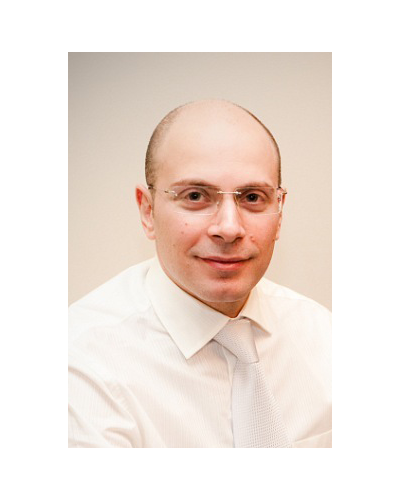
\includegraphics[width=35mm]{start1.png}
    \end{textblock*}
\end{frame}

\begin{frame}[t]
    \titlepage
    \begin{textblock*}{20mm}(0mm,5cm)%
      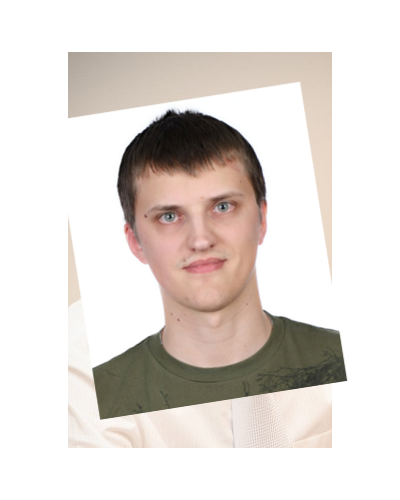
\includegraphics[width=35mm]{start2.png}
    \end{textblock*}
    \begin{textblock*}{20mm}(0.5\textwidth,3cm)%
      
\includegraphics[width=6cm]{stamp.png}
    \end{textblock*}
\end{frame}

\frame
{\frametitle{Disclaimer}
\begin{itemize}
  \item<2-> I'm not a Scala expert, actually, I do not know Scala at all.
  \item<3-> Lets discuss today not implementations, but ideas staying behind them.
\end{itemize}
}

\frame%
{\frametitle{Agenda}
  \tableofcontents[1]
}

\section{Parser combinators}
\frame
{\frametitle{XRools}
\begin{itemize}
  \item Written by Scala experts from Kiev
  \item XPath like DSL
  \item Extendable by Scala code
  \item XML oriented
\end{itemize}
}
\frame
{\frametitle{XRools}
\begin{center}
  \large Talk is cheap. Show me the code.
\end{center}
}
\subsection{XRools Pros}
\frame
{\frametitle{XRools Pros}
\begin{itemize}
    \item<1-> Scala
    \item<2-> Non-developers write rules
    \item<3-> Dashboard 
\end{itemize}
}
\subsection{XRools Cons}
\frame
{\frametitle{XRools Cons}
\begin{itemize}
    \item<1-> Scala
    \item<2-> Non-developers write rules
    \item<3-> No compile-time checks
    \item<4-> Uses reflection
    \item<5-> No real IDE support
    \item<6-> Not Turing-complete
    \item<7-> Functions defined away from its only usage
    \item<8-> Debugging?
\end{itemize}
}

\subsection{XRools}
\frame
{\frametitle{XRools}
  \begin{center}
    
\includegraphics[width=0.7\textwidth]{xrools.jpeg}
  \end{center}
}

\section{JAXB plugin}
\subsection{JAXB plugin}
\frame{
\frametitle{JAXB plugin}
\begin{itemize}
  \item Written by Sergey Armensky \\ (idea of Andrey Vytnov?)
  \item Plain Java (new method added for each property)
  \item Will be soon in production
  \item Have nothing to do with Scala
\end{itemize}
}
\frame
{\frametitle{JAXB plugin}
\begin{center}
  \large Talk is cheap. Show me the code.
\end{center}
}

\subsection{JAXB plugin Pros}
\frame{
\frametitle{JAXB plugin Pros}
\begin{itemize}
  \item<1-> Pure Java
  \item<2-> Simple and clean
  \item<3-> Simplify some code
\end{itemize}
}
\subsection{JAXB plugin Cons}
\frame{
\frametitle{JAXB plugin Cons}
\begin{itemize}
  \item<1-> Pure Java
  \item<2-> Only for JAXB generated classes
  \item<3-> Simplify only some code
  \item<4-> Not declarative enough
  \item<5-> Not mapper at all
\end{itemize}
}

\subsection{Can we do better?}
\frame{
\frametitle{JAXB Plugin}
  \begin{center}
    
\includegraphics[width=0.5\textwidth]{jaxb.jpg} 
  \end{center}
}
\frame{
\frametitle{Can we do better?}
  \begin{center} 
    \only<2-> {
      
\includegraphics[width=0.4\textwidth]{yajom.jpg} 
      \\~\\
      \large \textbf{CHALLENGE ACCEPTED}
    }
  \end{center}
}

\section{Scala Macros}
\subsection{Scala related features}
\frame
{\frametitle{Scala related features}
\begin{itemize}
  \item Implicits of all kinds
  \item Point-free style
  \item Scala virtualized
  \item Macros
\end{itemize}
}

\subsection{Yajom}
\frame
{\frametitle{Yajom}
\begin{itemize}
  \item Yet Another Java Object Mapper
  \item Based on implicits and Scala macros
  \item All reflection is done in compile-time
  \item Easy to configure, extend or derive \\ (having no clue about Scala Macros at all)
\end{itemize}
}

\frame
{\frametitle{Yajom}
\begin{center}
  \large Talk is cheap. Show me the code.
\end{center}
}

\subsection{Yajom Pros}
\frame{
\frametitle{Yajom Pros}
\begin{itemize}
  \item<1-> Scala
  \item<2-> Compile-time bulletproof
  \item<3-> IDE support
  \item<4-> I cannot imagine more declarative tool
  \item<5-> Works with any classes without any changes
  \item<6-> No problem with debugging
\end{itemize}
}
\subsection{Yajom Cons}
\frame{
\frametitle{Yajom Cons}
\begin{itemize}
  \item<1-> Scala
  \item<2-> Maybe not mature enough
  \only<3->{
    \begin{textblock*}{35mm}(0.8\textwidth,5cm)%
      
\includegraphics[width=35mm]{troll.png}
    \end{textblock*}
  }
\end{itemize}
}

\frame{\frametitle{Yajom}
  \begin{center}
    
\includegraphics[width=0.5\textwidth]{optocat.png}  \\
    \large \href{https://github.com/gark87/yajom}{https://github.com/gark87/yajom}
  \end{center}
}

\section{Q\&A, Discussion}
\frame{
  \begin{center}
    \Large Thank You!
  \end{center}
}

\end{document}
